% %% main.tex - AASTeX701 two-column final pass
\documentclass[twocolumn]{aastex701}

% ----- Packages (minimal) -----
\usepackage{amsmath, amssymb}
\usepackage{bm}
\usepackage{graphicx}
\graphicspath{{figs/}}
\usepackage[section]{placeins}
\usepackage{placeins}
\usepackage{needspace}
\usepackage{dblfloatfix}
\usepackage{balance}
\usepackage{flafter} % 図が参照より前に出ない保険


% 二段図の許容量を増やす(団子解消に効く)
\setcounter{dbltopnumber}{2}
\renewcommand{\topfraction}{.85}
\renewcommand{\floatpagefraction}{.7}

\makeatletter
\def\fps@figure{!htbp}
\def\fps@table{!htbp}
\makeatother

\hypersetup{colorlinks=true,linkcolor=blue,citecolor=blue,urlcolor=blue}
%\usepackage{array}
%\newcolumntype{L}[1]{>{\raggedright\arraybackslash}p{#1}}
% ----- Float tuning (tighter) -----
\setcounter{topnumber}{4}
\setcounter{bottomnumber}{3}
\setcounter{totalnumber}{6}
\setcounter{dbltopnumber}{1}

% 混雑ページだけ局所的にフロート数を絞る環境
\newenvironment{CrowdedFloats}{%
  \begingroup
  \setcounter{topnumber}{1}%
  \setcounter{totalnumber}{2}%
}{\endgroup}
% ===== end =====

\renewcommand{\topfraction}{0.97}
\renewcommand{\bottomfraction}{0.95}
\renewcommand{\textfraction}{0.05}
\renewcommand{\floatpagefraction}{0.70}
\renewcommand{\dbltopfraction}{0.88}
\renewcommand{\dblfloatpagefraction}{0.70}

\setlength{\floatsep}{4pt plus 1pt minus 1pt}
\setlength{\textfloatsep}{6pt plus 1pt minus 1pt}
\setlength{\intextsep}{4pt plus 1pt minus 1pt}
\setlength{\abovecaptionskip}{2pt}
\setlength{\belowcaptionskip}{1pt}

\raggedbottom

% ----- Macros -----
\newcommand{\ath}{a_{\rm th}}
\newcommand{\rg}{r_g}
\newcommand{\LEdd}{L_{\rm Edd}}
\newcommand{\Ltot}{L_{\rm tot}}
\newcommand{\FeKa}{\mathrm{Fe\,K}\alpha}
\newcommand{\epscoup}{\epsilon_{\rm coup}}
\newcommand{\aeq}{a_{\rm eq}}

% --- Compactness threshold (single source of truth) ---
\newcommand{\ellcrit}{30}
\newcommand{\ellhard}{\ell<\ellcrit}         % hard screen
\newcommand{\ellsoft}{\ell\lesssim\ellcrit}  % soft/typical statement

% tight enumerate/itemize (環境ラッパ・パッケージ不要)
\newenvironment{tenumerate}{%
  \begin{enumerate}\setlength{\itemsep}{0pt}\setlength{\parsep}{0pt}\setlength{\parskip}{0pt}%
}{\end{enumerate}}
\newenvironment{titemize}{%
  \begin{itemize}\setlength{\itemsep}{0pt}\setlength{\parsep}{0pt}\setlength{\parskip}{0pt}%
}{\end{itemize}}

% === one-liners(1つだけに統一) ===
% 置換(コロン版)
\DeclareRobustCommand{\tldr}[1]{%
  \noindent\textit{In brief:}~#1%
  \par\smallskip
  \noindent\rule{\columnwidth}{0.2pt}\par\medskip
}


\DeclareRobustCommand{\nav}[1]{%
  \noindent\textit{See also:}~#1\par\smallskip
}

% === Figure callout ===
\newcommand{\figcallout}[2]{%
  \noindent\begingroup\small\itshape
  \textbf{Figure~\ref{#1}}:\ #2\par
  \endgroup\vspace{2pt}%
}
% ----- PDF bookmark-safe strings -----
\PassOptionsToPackage{unicode}{hyperref}
\pdfstringdefDisableCommands{%
  \def\ath{a\_th}\def\rg{r\_g}\def\LEdd{L\_Edd}\def\Ltot{L\_tot}\def\FeKa{Fe K\string\alpha}%
  \def\epscoup{epsilon\_coup}\def\aeq{a\_eq}\def\mathrm#1{#1}%
}

% ----- Metadata -----
\shorttitle{Self-Sustained Penrose Excitation}
\shortauthors{Wakabayashi}

\begin{document}

\title{Self-Sustained Penrose Excitation of Accretion Disks:\\
A Spin-Regulated Mechanism for Super-Eddington Quasar Luminosities}
\correspondingauthor{Jun Wakabayashi}

\author[0009-0008-1891-4579]{Jun Wakabayashi}
\affiliation{Independent Researcher, Japan}
\email{waka132009@gmail.com}

\begin{abstract}
We present a high-spin, near-threshold equatorial radiative channel that (i) sustains super-Eddington luminosities and (ii) naturally enforces a sub-unity spin ceiling, explaining why spins do not exceed unity in practice. Compactness-limited transparency ($\ell$) gates the observable power, and a simple torque balance links the luminosity to the same control that sets the ceiling. The framework is immediately testable via three co-occurring hooks at high spin and high accretion rate: (1) a 20--120~keV high-energy shoulder favored over a featureless continuum by $\Delta$AICc or $\Delta$BIC $\ge 6$; (2) lag hardening from X to UV/optical; and (3) equator-aligned X-ray polarization with a rising degree. The path to falsification is explicit: in vetted high-spin, high-$\lambda$ quasars, failure to recover at least two hooks---after excluding heavy absorption, extreme inclination, and high-compactness cases---would refute the scenario.
\end{abstract}

\keywords{Quasars --- Accretion, accretion disks --- Black hole physics --- Relativistic processes}

% ===============================
% Executive Summary(5行)
% ===============================
\section*{Executive Summary}
\begin{tenumerate}
  \item Near-extremal spins enable a compactness-gated \emph{equatorial} radiative channel that sustains $L/L_{\rm Edd}>1$ while self-limiting the spin.
  \item The lever is repeated Penrose-like coupling at the ISCO-ergoregion interface, depositing power back into the disk and extracting angular momentum.
  \item The framework predicts three joint hooks: a hard X/MeV shoulder (20--120~keV, obs), lag hardening (X$\to$UV/optical), and equator-aligned X-ray polarization.
  \item Screens remove confounders: Compton-thick absorption, extreme inclination, and high compactness ($\ellhard$ required).
  \item \textbf{Kill-shot:} in vetted high-spin/high-$\lambda$ quasars, failure to recover $\ge\!2$ hooks (after screens) refutes the framework.
\end{tenumerate}

\section{Introduction}\label{sec:intro}
\tldr{Observed super-Eddington luminosities and sub-unity spin ceilings motivate an \emph{equatorial}, spin-regulated channel beyond viscous accretion alone.}
\noindent\textbf{Threshold, transparency, and a natural spin ceiling.}
Near-threshold activation at high spin, gated by compactness-limited transparency ($\ellsoft$), selects an equatorial radiative channel that both sustains $L/L_{\rm Edd}>1$ and imposes a spin ceiling.
This section sketches the mechanism and sets up testable consequences with explicit falsification (Eqs.~\eqref{eq:eps}--\eqref{eq:Ltot}; Fig.~\ref{fig:onset}).

Recent reviews have noted persistent tensions between thin--disk expectations and observations\textemdash{}
e.g., systematically large continuum-emitting sizes from microlensing and reverberation, and
wavelength-dependent lags exceeding simple reprocessing models \citep[e.g.,][]{Cackett2021RevMap,Sun2020AGNsize}.
These tensions motivate considering \emph{additional inner-disk heating} beyond local viscous dissipation.
Near $a_*\!\to\!1$, an \emph{equatorial, magnetically assisted Penrose-like split} provides a \emph{testable route}
to such reheating (Sec.~\ref{sec:mech-sketch}), with observational hooks and falsification criteria
(Sec.~\ref{sec:obs}).
The possibility of extracting rotational energy from the ergoregion was first pointed out by \citep{Penrose1969,Penrose2002}.


\paragraph{Scope and modeling stance.}
We present a phenomenological framework: the microphysics of beam formation, transport, and equatorial deposition is intentionally kept agnostic, while the \emph{observable consequences} of such coupling are made explicit and falsifiable. This stance allows clean confrontation with data now and provides a clear interface to future GRMHD/plasma studies that could instantiate the coupling agent.

\paragraph{Boundary conditions are not fixed near $a_*\!\to\!1$.}
Much of the literature treats the inner disk, magnetosphere, and ergoregion with effectively fixed cross-component boundary conditions. We instead emphasize that near-extremal spin the boundaries themselves evolve: frame dragging enlarges and reshapes the ergoregion, the ISCO approaches it, and the equatorial return path becomes thin and resistive. In this coupled regime an equatorial current sheet is generically required by the global field topology; shear and flux loading drive plasmoid-dominated reconnection; and the resulting split redistributes $(E,L)$ so that a negative-energy branch is absorbed by the hole while a gain branch vents as a narrow equatorial quasi-beam, part of which returns to heat the inner disk.


\section{Theoretical Framework}\label{sec:theory}
\tldr{Near-threshold Kerr coupling at the ISCO--ergoregion interface supplies disk heating while extracting spin, under a compactness gate $\ellhard$.}

\noindent All elements invoked below act outside the event horizon; the coupling operates in the ergoregion and deposits energy in the equatorial flow, avoiding assumptions about interior or singularity-scale physics.
\noindent\textit{Abbreviations and references.}
We use \emph{FFE} for the force-free, magnetically dominated limit ($\rho_e\mathbf{E}+\mathbf{J}\!\times\!\mathbf{B}\approx 0$, $\mathbf{J}\!\cdot\!\mathbf{E}=0$) and \emph{GRMHD} for ideal magnetohydrodynamics evolved on a Kerr background \citep{Komissarov2004MNRAS,GrallaJacobson2014MNRAS,EastYang2018PRD,Pan2018PRD}.
We use \emph{PIC} for first-principles kinetic simulations that resolve reconnection and plasmoid formation in the ergospheric current sheet \citep{Parfrey2019PRL,Bransgrove2021PRL}.
Throughout we group references as (FFE/GRMHD) versus (PIC).


\subsection{Kerr Energy Reservoir}\label{sec:kerr}
\tldr{A near-extremal Kerr hole stores $\sim0.29Mc^2$ of rotational energy that can power luminous episodes.}
For a Kerr black hole of mass $M$ and spin $a_\ast$, the extractable rotational energy is
\Needspace{12\baselineskip}
\begin{equation}
E_{\rm rot}(a_\ast)=\Bigg[1-\sqrt{\tfrac{1}{2}\Big(1+\sqrt{1-a_\ast^2}\Big)}\Bigg]\,Mc^2,
\label{eq:Erot}
\end{equation}
reaching $\sim0.29\,Mc^2$ as $a_\ast\to1$.

\subsection{Spin-Triggered Coupling}\label{sec:coupling}
\tldr{A steep activation above $a_{\rm th}\simeq0.97$ sets both the luminosity lever and a self-imposed spin ceiling.}
We posit a threshold spin $\ath$ above which an ergoregion-coupled agent activates. The effective coupling follows
\Needspace{7\baselineskip}
\begin{equation}
\epscoup(a_\ast)=
\begin{cases}
0, & a_\ast\le \ath,\\[3pt]
\epsilon_{\max}\Big(\dfrac{a_\ast-\ath}{1-\ath}\Big)^{n}, & a_\ast>\ath,
\end{cases}
\label{eq:eps}
\end{equation}
where $\epsilon_{\max}$ is the saturation cap and $n$ controls activation sharpness.
% === Figures tied to 3.2 (param space + onset) ===
\begin{figure}[!htbp]
  \centering
  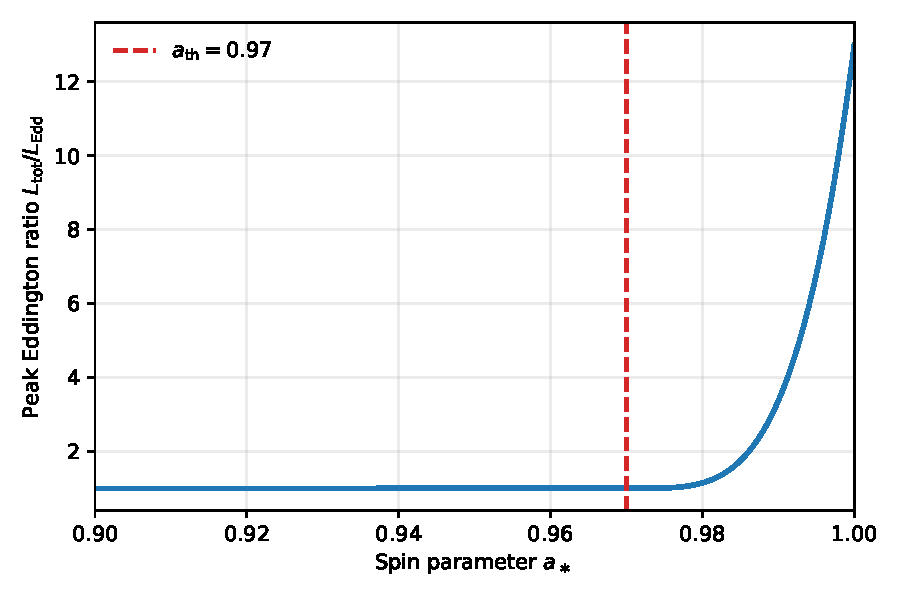
\includegraphics[width=.92\linewidth]{Fig_Onset.pdf}
\caption{\textbf{Activation turns on steeply above the threshold.}
Peak $\Ltot/\LEdd$ rises rapidly once $a_\ast\!>\!\ath$, setting the lever for luminosity and spin regulation (cf.\ Eqs.~\eqref{eq:eps}--\eqref{eq:Ltot}).}
  \label{fig:onset}
\end{figure}
% --- Takeaway first (3行以内) ---
\noindent\textit{Activation threshold.}
The equatorial coupling turns on steeply once the spin exceeds a threshold \(a_{\rm th}\).
In our fiducial calibration, the rise is rapid near \(a_\ast \simeq 0.97\), setting the lever for both luminosity boost and spin regulation (cf.\ Eqs.~\eqref{eq:eps}--\eqref{eq:Ltot}).
\FloatBarrier
Unless noted, we adopt the following fiducials for figures and estimates: $M=10^9M_\odot$, $\eta_{\rm acc}=0.1$, $\epsilon_{\max}=0.1$, $n=2$, $R_0=10^2$, and $\alpha=50$; the illustrative threshold is $\ath\simeq0.97$.
\noindent\emph{Micro-bridge.}
While we keep microphysics agnostic, the fiducial range
$\epsilon_{\rm coup}\sim10^{-2}$--$10^{-1}$ is broadly consistent with
energy-release fractions seen in near-horizon, plasmoid-dominated
reconnection in recent GRMHD studies. For the present framework we only
assume that $\epsilon_{\rm coup}$ rises sharply above $a_{\rm th}$ and
saturates below $\epsilon_{\max}$; detailed calibration is left for
future simulations.

\paragraph{Phenomenological parameters and physical ranges.}
The cap $\epsilon_{\max}$ limits equatorial deposition efficiency by energy-budget and pair-compactness constraints; $n$ controls activation sharpness above $\ath$ as an effective criticality index of the coupling geometry. $(R_0,\alpha)$ regulate the dissipation footprint to maintain transparency, trading compactness against reprocessing. We restrict these to physically plausible ranges and view them as interfaces for future GRMHD/plasma calibration, not curve-fitting knobs.
\paragraph{Sensitivity and saturation.}
The activation $\epsilon_{\rm coup}(a_*)$ is intentionally steep: $(a_{\rm th},n)$ set the narrowness of the “spin ceiling”. In practice $\epsilon_{\rm coup}$ and the leakage fraction depend nonlinearly on flux loading and $\dot M$, with possible saturation arbitrarily close to the extremal limit. We therefore treat $(a_{\rm th},n,\epsilon_{\max},\alpha)$ as calibration parameters to be fixed by future GRMHD-in-ergoregion testbeds.


\paragraph{Power partition.}
We allow the extracted rotational power to partition between a polar BZ jet and an equatorial feedback channel:
\[
P_{\rm ext}=P_{\rm jet}+P_{\rm eq},\qquad f_{\rm BZ}+f_{\rm eq}=1.
\]
Near $a_*\!\to\!1$, $f_{\rm eq}$ can become substantial (radio-quiet, radiation-dominated states), while $f_{\rm BZ}$ dominates in radio-loud systems; hybrid states are possible in transient MAD-like regimes.
%\FloatBarrier
\subsection{Mechanism sketch: a leaky equatorial return path}\label{sec:mech-sketch}
\tldr{Equatorial reconnection ejecta split in the ergoregion; a negative-energy branch is absorbed while a quasi-beam returns to heat the inner disk.}
\paragraph{Projectile sufficiency.}
Reconnection ejecta (plasmoids) in the ergoregion carry specific energy $E$ and angular momentum $L$. A Penrose split requires a branch with $E-\Omega_H L<0$ (horizon condition).\footnote{Notation follows Fig.~\ref{fig:equatorial_trigger}.}
Tension-driven redistribution during ejection changes $L$ by $\Delta L\!\sim\!\mathcal{O}(r_{\rm g}v_\phi)$ and reconnection outflows can reach $v\!\sim\!0.1$--$0.5c$ in high-$S$ sheets; hence tens-of-percent shifts in $L$ suffice to place a fraction on the negative-energy branch, with the complement forming the \emph{positive-energy branch} (equatorial quasi-beam).
Near-extremal spin brings the ISCO into close contact with the ergoregion and enforces an equatorial return current sheet at their interface. Shear and flux loading thin the sheet until it becomes tearing-unstable; reconnection then ejects plasmoids as a chain of narrow, equator-following pulses. These ejecta provide the “projectile” required by a Penrose-like energy split: within the ergoregion, a fraction of the flow is placed on negative-energy-at-horizon trajectories while the counterpart gains energy and escapes. The extraction condition is simply
\begin{equation}
E - \Omega_H L < 0 \, .
\label{eq:penrose-cond}
\end{equation}
\noindent cf.\ \citealt{Penrose1969,Penrose2002}.
so the black hole’s rotational energy pays for the escaping branch. The centrifugal barrier and toroidal tension form an equatorial nozzle, so a growing fraction of the circuit power vents as a collimated equatorial quasi-beam while the DC return still closes globally. A modest back-flow coupling ($\epsilon_{\rm coup}\!\sim\!10^{-2}$--$10^{-1}$) suffices to heat the inner disk and regenerate magnetic flux, closing a self-sustained loop. The active zone and leakage fraction increase monotonically with spin (and also depend nonlinearly on flux loading and accretion rate), with possible saturation arbitrarily close to the extremal limit.
% 節頭直後に図が先出しされるのを抑止したい場合は次を追加:
% \suppressfloats[t]
\begin{figure*}[p!]
  \centering
  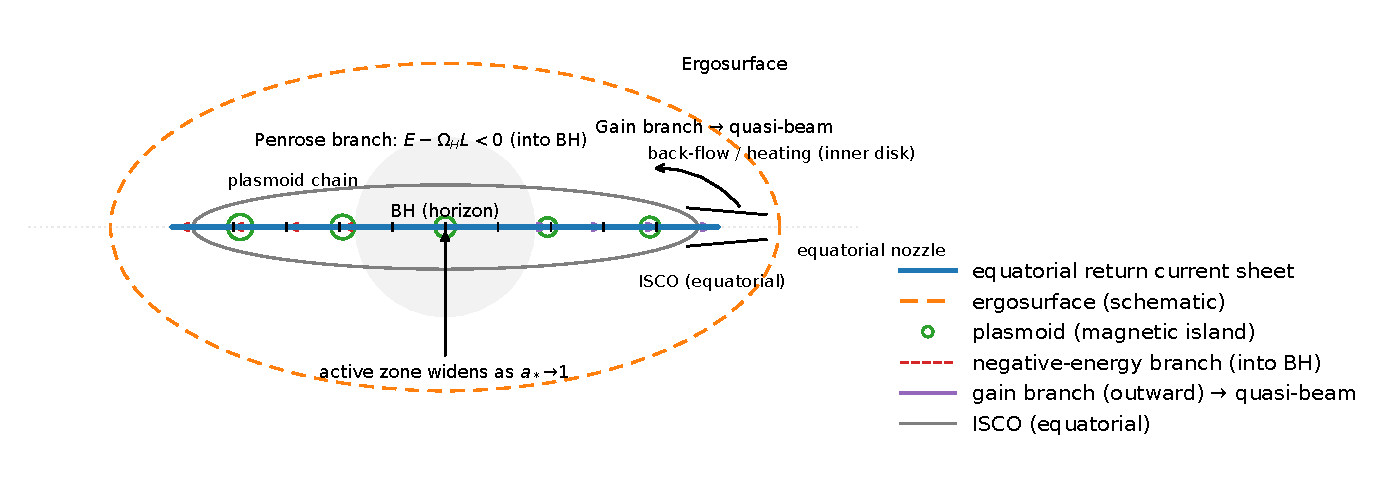
\includegraphics[width=\textwidth]{fig_equatorial_trigger_schematic.pdf}
  \caption{\textbf{Equatorial Penrose trigger: negative vs.\ positive branches.}}
  Plasma from the inner disk/plunging region enters the ergosphere and splits kinematically:
  a \emph{negative-energy branch} with $E-\Omega_H L<0$ falls through the \emph{event horizon} ($r_{\rm H}$),
  while a \emph{positive-energy branch} emerges as an equatorial quasi-beam that reheats the inner rim near $r_{\rm ISCO}$ \citep{Penrose1969,Penrose2002}.
  Landmarks\textemdash{}ergosurface, $r_{\rm ISCO}$, and the equatorial return current sheet (blue ribbon)\textemdash{}are indicated; branches are shown as \emph{red solid} (positive) and \emph{blue dashed} (negative) to match Eq.~\eqref{eq:penrose-cond}.
  
  {\footnotesize(FFE/GRMHD: \citealt{Komissarov2004MNRAS,EastYang2018PRD,Pan2018PRD};
                 PIC: \citealt{Parfrey2019PRL,Bransgrove2021PRL}).}
  \label{fig:equatorial_trigger}
\end{figure*}
% 小節を跨いで流れないように必要なら1回だけ:
\FloatBarrier

\paragraph{Why an equatorial, quasi-collimated branch?}
Near $a_*\!\to\!1$ the combination of (i) the equatorial centrifugal barrier,
(ii) strong toroidal fields generated by shear (hoop stress), and
(iii) pressure deficits carved by intermittent reconnection outflows
forms an ``equatorial nozzle''. The \emph{positive-energy branch} therefore propagates as a
narrow, radiation-supported quasi-beam rather than escaping along the poles.
Because the transport remains largely collisionless/Poynting-dominated until
it reprocesses in the inner disk, and because the dissipation footprint is
extended ($R_{\rm eff}\!\sim\!10^{2}$--$10^{3}\,r_g$), the pair compactness
along the beam stays low, consistent with the transparency requirement of Eq.~(6).

%\FloatBarrier
\subsection{Self-Sustained Penrose Excitation}\label{sec:penrose}
\tldr{A modest feedback fraction $\epsilon_{\rm coup}\sim10^{-2}\!-\!10^{-1}$ closes the loop, sustaining bright states without pair-choking.}
The mean extraction power is $\langle P_{\rm ext}\rangle=E_{\rm rot}/\tau$, and with duty cycle $d$ the instantaneous power during active phases is $P_{\rm ext}\sim\langle P_{\rm ext}\rangle/d$. Here $\tau$ denotes the effective extraction e-folding timescale of the rotational-energy reservoir, i.e., $\langle P_{\rm ext}\rangle=E_{\rm rot}/\tau$ using Eq.~\eqref{eq:Erot}.
%\FloatBarrier
\subsection{Disk Dissipation and Scale}\label{sec:diss}
\tldr{An extended footprint $R_{\rm eff}\sim10^2\!-\!10^3\,r_g$ keeps $\ell$ low so the hard component remains transparent.}
A fraction $\epscoup(a_\ast)$ of $P_{\rm ext}$ is deposited into the disk:
\begin{equation}
L_{\rm self}=\epscoup\,P_{\rm ext},
\label{eq:Lself}
\end{equation}
and the dissipation spreads over an effective radius
\paragraph{Self-transparency (physical note).}
The scaling $R_{\rm eff}\!\approx\!R_0[1+\alpha(\epsilon_{\rm coup}/\epsilon_{\max})]\,r_{\rm g}$ phenomenologically captures geometric spreading, multi-zone deposition, and increased scattering mean free paths as the equatorial quasi-beam heats and rarefies the inner disk corona. Our results require $R_{\rm eff}\!\sim\!10^2$--$10^3\,r_{\rm g}$ during bright episodes to keep the pair compactness low (cf. Sec.~\ref{sec:transp}).
\begin{equation}
R_{\rm eff}\approx R_0\Big[1+\alpha\Big(\frac{\epscoup}{\epsilon_{\max}}\Big)\Big]\,\rg,
\label{eq:Reff}
\end{equation}
with $\rg=GM/c^2$, fiducial $R_0\sim10^2$ and $\alpha\sim50$.

%\FloatBarrier
\subsection{Transparency (Compactness Constraint)}\label{sec:transp}
\tldr{Transparency requires $\ellsoft$, linking power deposition to geometry and spectrum.}
Transparency requires pair compactness
\begin{equation}
\ell=\frac{L_{\rm self}\sigma_T}{4\pi R_{\rm eff}\,m_e c^3}\lesssim\ellcrit,
\label{eq:ell}
\end{equation}
which couples Eqs.~\eqref{eq:Lself} and \eqref{eq:Reff} and motivates $R_{\rm eff}\sim10^2$--$10^3\,\rg$ during bright episodes.  
\textit{We adopt $\ellsoft$ as a conservative transparency threshold following classic compactness arguments; the precise value depends on geometry and spectrum and can be re-tuned in data applications. See, e.g., \citep{1984MNRAS.209..175S,LightmanZdziarski1987}.}

%\FloatBarrier
\subsection{Spin and Mass Evolution}\label{sec:evol}
\tldr{Torque balance with $\Omega_H$ enforces $a$-drift toward an equilibrium $a_{\rm eq}$ below unity.}
The horizon angular frequency is
\begin{equation}
\Omega_H=\frac{a_\ast c^3}{2GM\big(1+\sqrt{1-a_\ast^2}\big)},
\label{eq:OmegaH}
\end{equation}
where $r_H=\rg\big(1+\sqrt{1-a_\ast^2}\big)$ and $\rg=GM/c^2$.
Evolution obeys
\begin{align}
\frac{dM}{dt}&=\frac{dM_{\rm acc}}{dt}-\frac{P_{\rm ext}}{c^2},\label{eq:dM}\\
\frac{dJ}{dt}&=\frac{dJ_{\rm acc}}{dt}-\frac{P_{\rm ext}}{\Omega_H},\label{eq:dJ}\\
\frac{da_\ast}{dt}&=\frac{c}{GM^2}\frac{dJ}{dt}-2a_\ast\frac{1}{M}\frac{dM}{dt}.\label{eq:da}
\end{align}

% === Figures tied to 3.6 (torque balance + spin track) ===
\begin{CrowdedFloats}
\begin{figure}[!htbp]
  \vspace*{2pt}
  \centering
  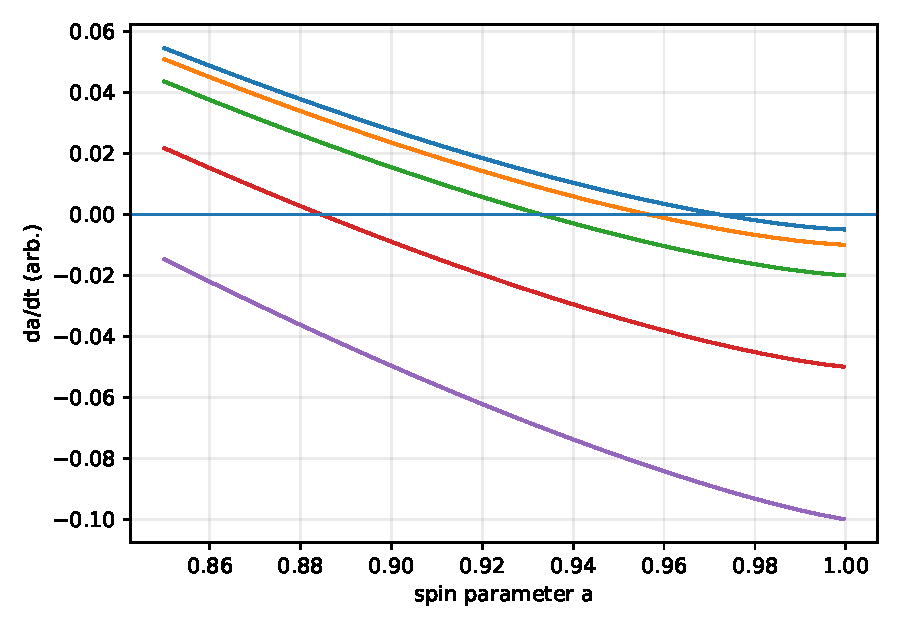
\includegraphics[width=.95\linewidth]{Fig3a.pdf}\\[4pt]
  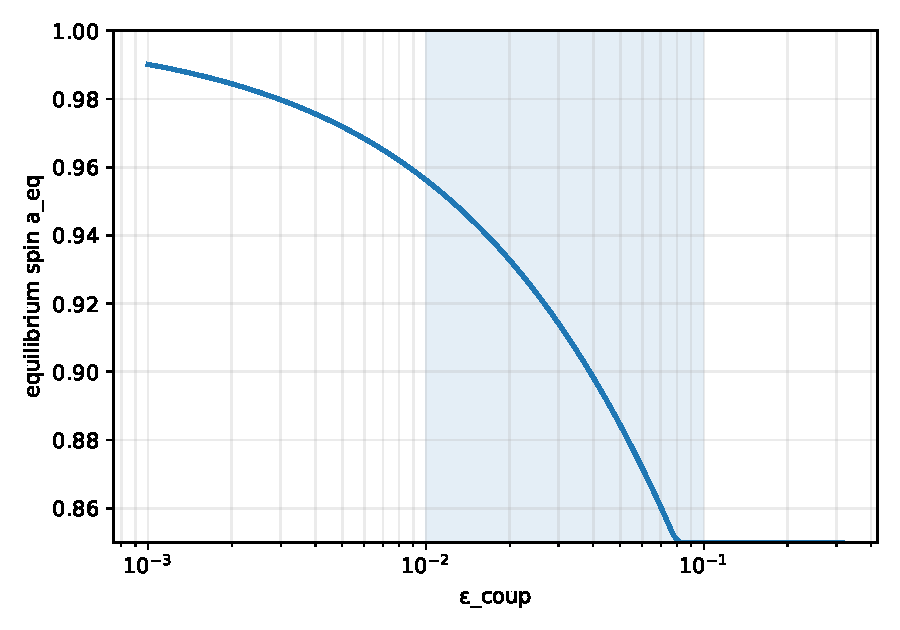
\includegraphics[width=.95\linewidth]{Fig3b.pdf}
  \caption{\textbf{Spin evolution and equilibrium vs.\ coupling.}
  \emph{Top:} Spin drift rate $da_\ast/dt$ from Eqs.~(\ref{eq:dM})--(\ref{eq:da}) for representative accretion states; negative values drive $a_\ast$ below unity.
  \emph{Bottom:} Equilibrium spin $a_{\rm eq}$ obtained from $da_\ast/dt=0$ as a function of $\epsilon_{\rm coup}$; ... the shaded band $\epsilon_{\rm coup}\sim10^{-2}$--$10^{-1}$ is the fiducial range used elsewhere. See also Eq.~(\ref{eq:OmegaH}).}
  \label{fig:fig3}
\end{figure}

\begin{figure}[!htbp]
  \centering
  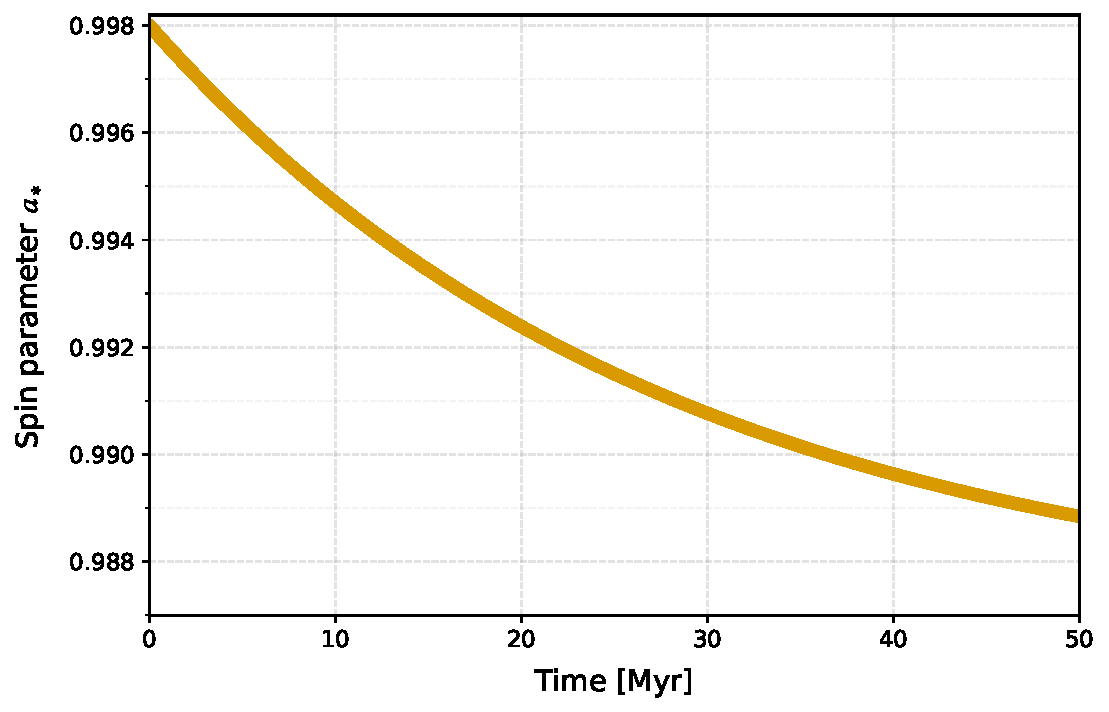
\includegraphics[width=\columnwidth,height=0.36\textheight,keepaspectratio]{fig2a_spin_evolution.pdf}
  % Fig.4(時間発展:スピンダウン)
  \caption{\textbf{Spin-down on Myr scales under equatorial extraction.}
  Time evolution of the spin parameter $a_\ast(t)$ obtained by integrating
  Eqs.~(\ref{eq:dM})--(\ref{eq:dJ})--(\ref{eq:da}) with horizon frequency \eqref{eq:OmegaH}
  for a fiducial coupling $\epsilon_{\rm coup}$ (gold). The monotonic drift toward
  $a_{\rm eq}<1$ illustrates the self-limiting ceiling; see Sec.~\ref{sec:discussion}.}
  \label{fig:spin-evo}
\end{figure}
\end{CrowdedFloats}
%\FloatBarrier
\subsection{Net Luminosity}\label{sec:lum}
\tldr{Total luminosity combines accretion and equatorial feedback, naturally yielding $L/L_{\rm Edd}\sim2$--$3$.}
The total luminosity is
\begin{equation}
\Ltot=L_{\rm acc}+L_{\rm self},\qquad
L_{\rm acc}\approx \eta_{\rm acc}\,\Big(\frac{dM_{\rm acc}}{dt}\Big)c^2,
\label{eq:Ltot}
\end{equation}
which links the dynamical solution (Eqs.~\eqref{eq:dM}--\eqref{eq:da}) to observables.

\paragraph{Energetic sanity check (one-line).}
With $M_{\rm BH}=10^9\,M_\odot$ [$Mc^2\simeq1.8\times10^{63}$ erg] and $E_{\rm rot}\!\sim\!0.1\,Mc^2$, a reservoir e-fold $\tau=10^7$ yr, $\epscoup=0.05$, and duty $d=0.2$ yield 
$L_{\rm self}\!\sim\!(E_{\rm rot}/\tau)\,(\epscoup/d)\!\approx\!1.4\times10^{47}\,{\rm erg\,s^{-1}}\!\sim\!1.1\,\LEdd$,
and $2$--$3\,\LEdd$ when combined with concurrent accretion, while $da_\ast/dt<0$ prevents overspin.

% === Figures tied to 3.7 (timescale + L mapping) ===
%\Needspace{18\baselineskip}$
\begin{figure}[!htbp]
  \vspace*{2pt}
  \centering
  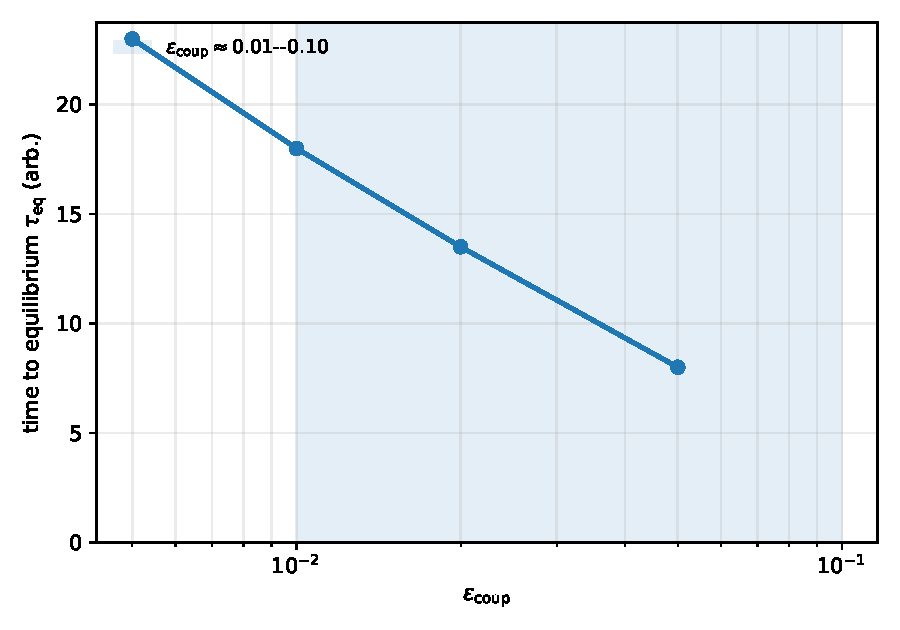
\includegraphics[width=.95\linewidth]{Fig4a.pdf}\\[4pt]
  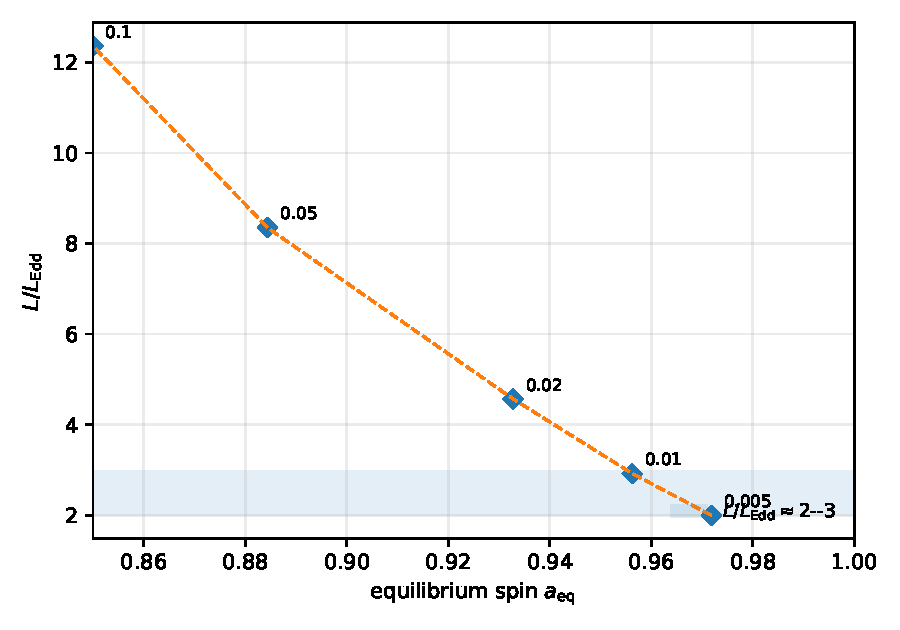
\includegraphics[width=.95\linewidth]{Fig4b.pdf}
  \caption{\textbf{Equilibrium timescale and luminosity mapping.}
  \emph{Top:} Time to equilibrium $\tau_{\rm eq}$ versus coupling $\epsilon_{\rm coup}$,
  computed from the spin-evolution system Eqs.~(\ref{eq:dM})--(\ref{eq:da}) with horizon frequency \eqref{eq:OmegaH};
  the shaded band $\epsilon_{\rm coup}\sim10^{-2}$--$10^{-1}$ is the fiducial range used elsewhere.
  \emph{Bottom:} Total luminosity at equilibrium, $L_{\rm tot}/L_{\rm Edd}$ from Eq.~(\ref{eq:Ltot}) evaluated at $a_\ast=a_{\rm eq}$,
  showing a typical $2$--$3$ band (blue) with labeled $\epsilon_{\rm coup}$ values along the trend.}
\end{figure}

\section{Results}\label{sec:results}
\tldr{Model trends map directly to hooks; figures follow their defining equations to prevent misalignment.}


The figures embedded in Sec.~\ref{sec:theory} visualize each theoretical ingredient immediately after the defining equations to avoid misalignment between formulae and diagnostics. Here we summarize cross-implications and observational hooks.

\clearpage
\subsection{Observational Hooks}\label{sec:obs}
\tldr{After screens, three hooks: MeV shoulder, lag hardening, and equator-aligned polarization\textemdash{}should co-occur in the bright, high-spin subset.}
\suppressfloats[t]  % avoid a float jumping above the heading

\noindent\textit{Why this matters.} What to look for and how to falsify, in plain terms.

% --- Quick recall of the equations each plot is tied to (往復を減らす) ---
\noindent\textit{Recall.}
Activation $\epsilon_{\rm coup}(a_\ast)$ and power $P_{\rm eq}=\epsilon_{\rm coup}\,\dot{M}c^2\,g(\ell)$
(cf.\ Eqs.~\eqref{eq:eps}, \eqref{eq:Ltot}), with transparency set by compactness $\ell$ (Eq.~\eqref{eq:ell}).
These establish the trends in the plots below.

\noindent\textbf{Screens (apply first).}
Exclude heavy absorption (Compton-thick etc.), extreme inclination, and high compactness ($\ell\gtrsim\ellcrit$).

\noindent\textbf{Hooks (apply jointly under the screens).}
\begin{titemize}
  \item \textbf{Hard X/MeV shoulder (20--120 keV, obs):}
        model comparison favors a shoulder over a featureless baseline by
        $\Delta$AICc \emph{or} $\Delta$BIC $\ge 6$
        (rest $\sim$0.3--1~MeV at $z\gtrsim6$).
  \item \textbf{Lag hardening (X$\to$UV/optical):}
        energy-resolved lags increase \emph{monotonically} with photon energy within an epoch.
  \item \textbf{Equator-aligned X-ray polarization (2--10~keV):}
        EVPA $\parallel$ equator; polarization degree increases toward high spin/high $\lambda$.
\end{titemize}

\noindent\textbf{Falsification.}
In vetted high-spin, high-$\lambda$ quasars, \emph{failure to recover at least two hooks} after the screens above \emph{refutes} the framework.
% --- 図はトップ優先で近くに出す ---
\begin{figure}[t!]
  \vspace*{2pt}
  \centering
  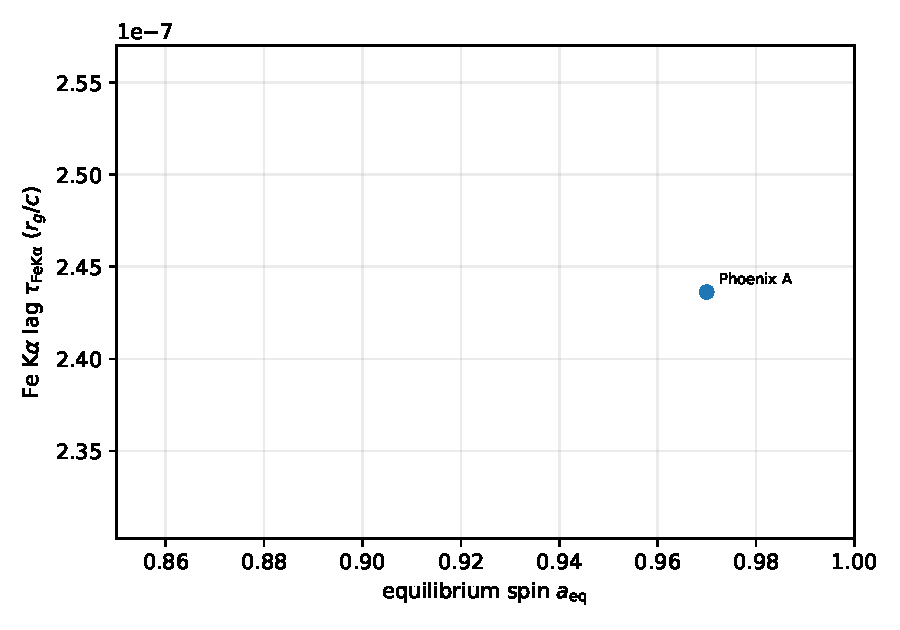
\includegraphics[width=.49\columnwidth]{Fig5a.pdf}
  \hfill
  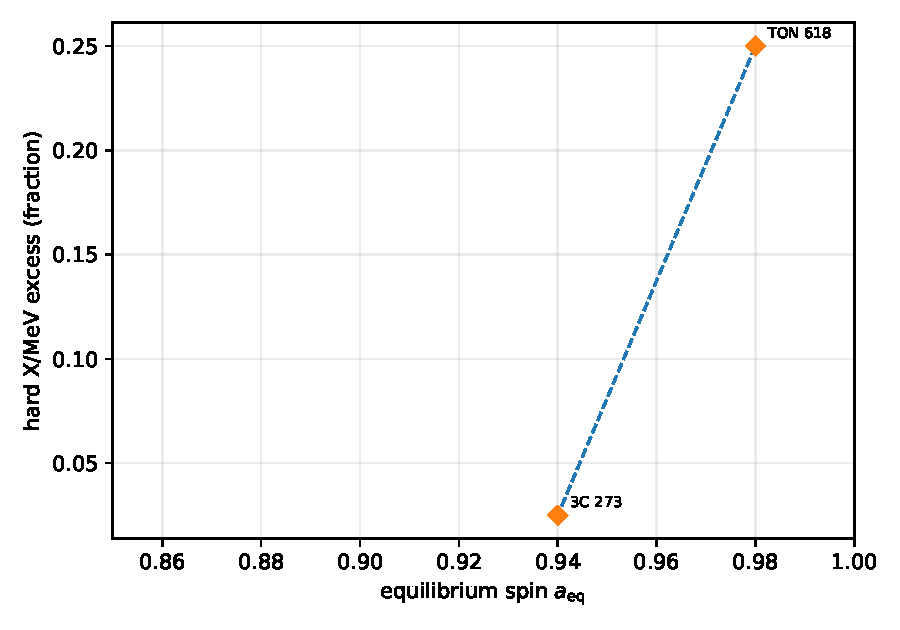
\includegraphics[width=.49\columnwidth]{Fig5b.pdf}
  \caption{\textbf{Hook observables vs.\ equilibrium spin.}
  \emph{Left:} Fe K$\alpha$ reverberation lag $\tau_{\rm FeK}$ (in $r_g/c$) as a function of $a_{\rm eq}$; lags increase toward lower $a_{\rm eq}$ (stronger coupling).
  \emph{Right:} Observable fraction $f_{\rm hook}$ (hard X/MeV shoulder or 2--10~keV polarization) vs.\ $a_{\rm eq}$ from the toy population mapping; the fraction rises steeply toward low $a_{\rm eq}$.
  See Sec.~\ref{sec:obs} and App.~\ref{app:protocol} for definitions and pass criteria.}
  \label{fig:fig5}
\end{figure}

%\FloatBarrier
\noindent\textit{At a glance.} How power repartitions at high $\lambda$ across mechanisms.

\floattable
\begin{deluxetable*}{lccc}[t] % ← ★付き+[t]で上部固定(専用ページなら [p])
\tablenum{1}
\tablecaption{\textbf{Bottom line:} the equatorial channel sustains $L/L_{\rm Edd}\!>\!1$ \emph{and} imposes a spin ceiling $a_{\rm eq}\!\approx\!a_{\rm th}$, complementary to slim-disk (no ceiling) and BZ/MAD (polar power, $a_{\rm eq}\!\sim\!0.5$--$0.7$).\label{tab:mech-contrast}}
\tabletypesize{\footnotesize}
\tablewidth{0pt}
\tablehead{
  \colhead{} & \colhead{$L/L_{\rm Edd}>1$} & \colhead{spin ceiling} & \colhead{channel}
}
\startdata
Slim disk        & yes (advective)                  & no                               & radiation (disk) \\
BZ/MAD           & indirect                         & yes ($a_{\rm eq}\sim0.5$--$0.7$) & polar Poynting (jet) \\
\textbf{This work} & \textbf{yes (equatorial)}         & \textbf{yes ($a_{\rm eq}\approx a_{\rm th}$)} & \textbf{equatorial Penrose-like} \\
\enddata
\end{deluxetable*}
% (必要なら直前に一度だけ) 
\FloatBarrier
%\suppressfloats[b]

\clearpage
%\Needspace{10\baselineskip} 
\section{Discussion}\label{sec:discussion}
\tldr{The equatorial branch complements polar BZ; an anti-correlated see-saw is expected across states.}
These bounds align with Fig.~\ref{fig:param-a}--\ref{fig:param-b} and are sufficient to reach $L/\LEdd\sim2$--$3$ with rarer $5$--$10\times$ excursions. Slim disks allow modest super-Eddington flows but no spin ceiling. BZ/MAD explain jet power yet not the radiative dominance of radio-quiet quasars. This framework ties hyperluminous output and the spin ceiling via near-extremal, equatorial coupling.
Consistent with GRFFE/GRMHD studies, an \emph{equatorial return-current sheet forms within the ergoregion} and becomes plasmoid-unstable; detached plasmoids naturally split into branches with $E-\Omega_H L\lessgtr 0$ (captured vs.\ escaping), enabling rotational-energy extraction via a Penrose-like radiative channel \citep{Penrose1969,Penrose2002,Komissarov2004MNRAS,EastYang2018PRD,Pan2018PRD,Parfrey2019PRL,Bransgrove2021PRL}.


%\medskip
\noindent\textit{Relation to Blandford--Znajek jets.}
BZ is polar/Poynting-dominated; our mechanism is equatorial/radiative. Hybrid states and an anti-correlated see-saw are expected; counterexamples (simultaneously strong jets and high radiative output) can occur in transitional MAD-like regimes.

% --- Parameter-space (panel a) : make it slightly shorter to allow text insertion ---
\begingroup
\setlength{\textfloatsep}{6pt plus 2pt minus 2pt} % 図まわりの余白を局所的に詰める
\begin{figure}[tp!]
  \centering
  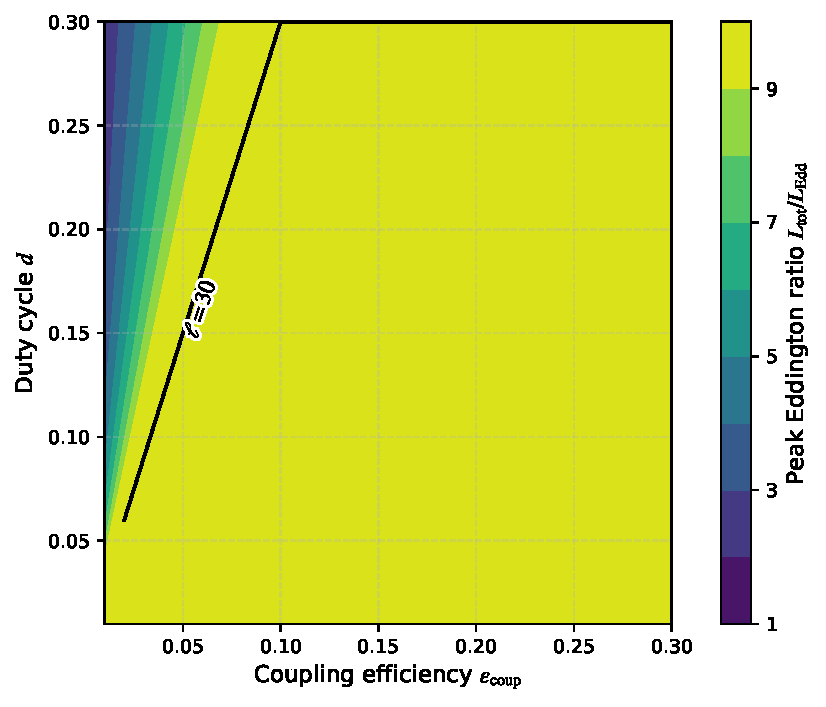
\includegraphics[width=0.95\columnwidth,trim=0 6 0 4,clip]{fig10a_Reff100.pdf}
  \vspace{-2pt}
  \caption{\textbf{Transparency selects the viable high-luminosity regime.}
  Peak Eddington ratio $L_{\rm tot}/L_{\rm Edd}$ (color) on the $(\epsilon_{\rm coup},d)$ plane; the black contour marks $\ell{=}\ellcrit$ from Eq.~(\ref{eq:ell})
  with components defined in Eqs.~(\ref{eq:Lself},\ref{eq:Reff}). For $R_{\rm eff}=100\,r_g$, the allowed region lies \emph{outside} the $\ell{=}\ellcrit$ contour, where
  $L_{\rm tot}/L_{\rm Edd}\sim2$--$3$ is typical with rarer $5$--$10\times$ excursions; see App.~\ref{app:protocol}.}
  \label{fig:param-a}
\end{figure}
\endgroup
% --- Parameter-space (panel b) : make it slightly shorter to allow text insertion ---
\begin{figure}[tp!]
  \centering
  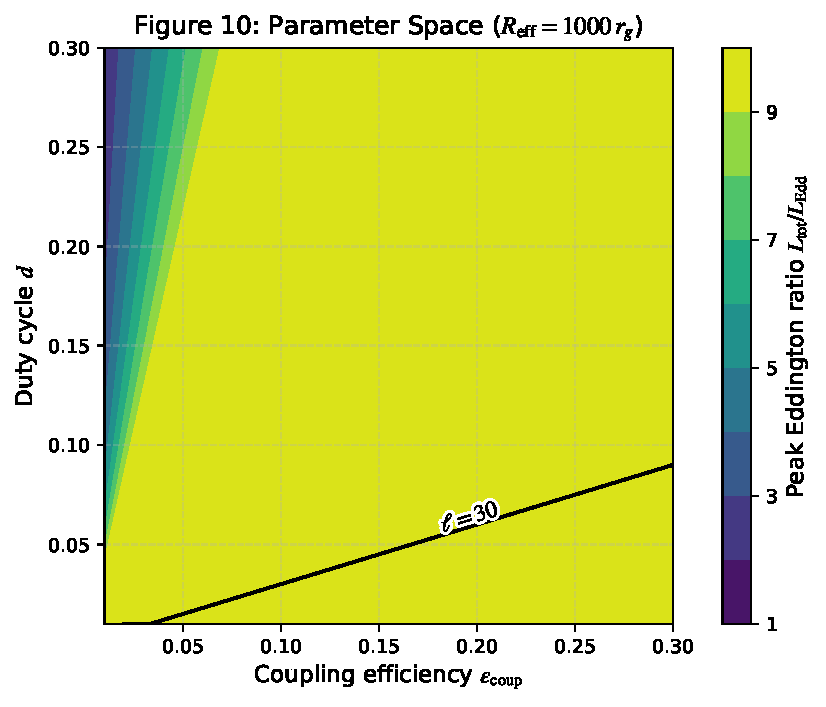
\includegraphics[width=0.95\columnwidth,trim=0 6 0 4,clip]{fig10b_Reff1000.pdf}
  \vspace{-2pt}
  \caption{\textbf{A larger dissipation footprint widens the transparent window.}
  Peak $L_{\rm tot}/L_{\rm Edd}$ (color) on the $(\epsilon_{\rm coup},d)$ plane for a larger footprint $R_{\rm eff}=1000\,r_g$.
  The $\ell{=}\ellcrit$ boundary (black; from Eq.~(\ref{eq:ell}) with components in Eqs.~(\ref{eq:Lself},\ref{eq:Reff})) shifts so that
  higher peaks in $L_{\rm tot}/L_{\rm Edd}$ remain compactness-safe, enlarging the viable region compared to Fig.~\ref{fig:param-a}.}
  \label{fig:param-b}
\end{figure}

\FloatBarrier


\paragraph{Power partition between polar and equatorial channels.}
We model the spin-extraction power as a partition between a polar Blandford--Znajek (BZ) channel and an equatorial feedback channel,
% amsmath は AASTeX で既定読み込み。無ければ \usepackage{amsmath}
\begin{align}
P_{\rm tot} &= P_{\rm BZ} + P_{\rm eq}, \\
P_{\rm BZ}  &= f_{\rm BZ}\,P_{\rm ext}, \qquad
P_{\rm eq} = f_{\rm eq}\,P_{\rm ext}, \\
f_{\rm BZ} + f_{\rm eq} &= 1.
\end{align}

This partition predicts an anti-correlation between radio-jet dominance and equatorial reheating diagnostics within the high-$a_*$, high-$\lambda$ subset, with hybrid states possible in transient MAD phases.
Our claim is modest: in the high-spin, high-Eddington subset, $f_{\rm eq}$ is statistically non-zero and sometimes dominant; in others, $f_{\rm BZ}$ may prevail. Outside this subset we make no claim.

\subsection*{Validation roadmap: observations and simulations}
% --- Validation Roadmap(置換用) ---
\subsection{Validation Roadmap}\label{sec:roadmap}
\tldr{Polarization--spin trends, intra-epoch lag slopes, and compactness screens lead; GRMHD+RT+population studies anchor the pipeline.}

\noindent\textbf{Observational fronts.}
\begin{enumerate}
  \item[\textbf{(i)}] \textit{\textbf{Polarization vs.\ spin.}}Test that EVPA is equator-aligned and that the degree rises with $a_\ast$/$\lambda$; control for jet and scattering-cone geometries; report rank-correlation $p$-values and effect sizes.
  \item[\textbf{(ii)}] \textit{\textbf{Lag hardening.}} Within single epochs, verify that X$\to$UV/optical lags increase monotonically with photon energy; mask absorption events; provide cadence/noise tests.
  \item[\textbf{(iii)}] \textit{\textbf{Spectral compactness screen.}} Use cutoff-energy/pair proxies to flag high-$\ell$ cases (non-transparent) and separate them from the transparent sample used for hooks.
  \item[\textbf{(iv)}] \textit{\textbf{See-saw with BZ.}} In jet-dominated sources, test anti-correlation between polar Poynting dominance and equatorial radiative signatures across states.
\end{enumerate}

\noindent\textbf{Simulation fronts.}
\begin{enumerate}
  \item[\textbf{(i)}] \textit{GRMHD near the ergoregion.} Resolve the equatorial return current sheet; quantify energy partition into positive/negative branches ($E-\Omega_H L\gtrless 0$); compare with torque-balance trends.
  \item[\textbf{(ii)}] \textit{Radiative transfer with pairs.} Propagate hard X/MeV emission through compactness-limited media; map when the shoulder survives vs.\ is quenched (link to $\ell$ cut).
  \item[\textbf{(iii)}] \textit{Population modeling.} Combine spin distributions with transparency and coupling priors to predict the fraction of sources passing $\ge 2$ hooks.
\end{enumerate}

%\noindent\textbf{Failure mode (falsification).}
%In vetted high-spin, high-$\lambda$ samples, absence of $\ge 2$ hooks after the transparency/absorption/inclination screens refutes the framework.
% --- ここまで ---

\paragraph{What would falsify this framework (kill shots).}
We explicitly delineate outcome patterns under which the equatorial channel is unnecessary. In the high-spin, high-$\lambda$ subset (e.g., $a_*\gtrsim0.8$, $\lambda\!\equiv\!L_{\rm bol}/L_{\rm Edd}\gtrsim0.3$), any of the following, if established \emph{as a population trend}, would falsify our claim:
\begin{enumerate}
\item Systematic absence of the EUV/soft-X/MeV excess (no ``shoulder'') \emph{and} systematically weak high-ionization lines (He\,II, N\,V, C\,IV) relative to the parent population.
\item Reverberation lags from X$\rightarrow$UV showing no energy dependence (no inward reheating signature).
\item $L_{\rm bol}$ not anti-correlated (even weakly) with $a_*$ within the bright subset (no self-regulated spin-down imprint).
\item Optical/X-ray polarization failing to favor equatorial angles or degrees when near-threshold spins are inferred.
\end{enumerate}
If \emph{two or more} items above hold simultaneously for the same high-spin, high-$\lambda$ subset, we would consider $f_{\rm eq}\!\to\!0$ supported and this mechanism unnecessary.

\section{Conclusion}\label{sec:conclusion}
\tldr{Recovering $\ge2$ hooks under screens supports the framework; systematic absence in high-spin/high-$\lambda$ would falsify it.}
Self-sustained Penrose excitation near extremal Kerr SMBHs can inject rotational energy into the accretion disk, yielding sustained $2$--$3\times$ Eddington with rarer $5$--$10\times$ episodes while enforcing a spin ceiling.

% ---------------- Appendix ----------------
\clearpage
\appendix

\section{Operational Protocol (Self-contained)}\label{app:protocol}
\noindent\textbf{Screens.} Exclude Compton-thick, extreme inclination; require $\ell<\ellcrit$.\\
\noindent\textbf{Hook (i):} Shoulder passes if $\Delta$AICc \emph{or} $\Delta$BIC $\ge 6$ (20--120~keV obs).\\
\noindent\textbf{Hook (ii):} Lag hardening passes if $d\tau/d\log E>0$ and monotone within an epoch.\\
\noindent\textbf{Hook (iii):} X-ray polarization: EVPA $\parallel$ equator; degree increases with spin/$\lambda$.\\
\noindent\textbf{Verdict.} After screens, absence of $\ge2$ hooks $\Rightarrow$ falsified; else passes.


\floattable
\begin{deluxetable*}{lcccc}[p]   % [t]で上部固定。収まらなければ[p]に
\tablewidth{0pt}
\tabletypesize{\normalsize}           % 大きく見せたい:\normalsize / 収めたい:\scriptsize
\tablecaption{\textbf{Candidate Gallery} \textemdash{} Representative objects; values are indicative.\label{tab:cands}}
\tablehead{
  \colhead{Name} & \colhead{$z$} &
  \colhead{$M_{\rm BH}/M_\odot$} & \colhead{$L/L_{\rm Edd}$} &
  \colhead{Notes}
}
\startdata
TON 618        & 2.219 & $\sim6.6\times10^{10}$ & $\sim3$     & \parbox[t]{0.36\textwidth}{Extremely massive; radio-loud; literature refs.\tablenotemark{a}}\\
J2157-3602     & 4.75  & $\sim3.4\times10^{9}$  & $\gtrsim10$ & \parbox[t]{0.36\textwidth}{Hyper-luminous; super-Eddington episode indications.\tablenotemark{b}}\\
J0100+2802     & 6.30  & $\sim1.2\times10^{10}$ & $\sim2$     & \parbox[t]{0.36\textwidth}{$z>6$ luminous quasar.\tablenotemark{c}}\\
J0439+1634     & 6.51  & $\sim7\times10^{9}$    & $\sim2{-}3$ & \parbox[t]{0.36\textwidth}{Possible lensing history.\tablenotemark{d}}\\
\enddata
\tablecomments{Values are illustrative; per-object sourcing is out of scope.}
\tablenotetext{a}{Virial-factor dominated systematics; radio-loud bias possible.}
\tablenotetext{b}{Bolometric/line-width systematics $\gtrsim 0.3$ dex.}
\tablenotetext{c}{High-$z$ mass methods differ (reflection vs.\ continuum).}
\tablenotetext{d}{Historical lensing debate; values assume de-lensing consensus.}
\end{deluxetable*}

\FloatBarrier
\section*{Cautionary note.}
Claims here are modular and falsifiable. Alternative mechanisms may dominate in other classes.

\section*{Author contributions}
Conceptualization, modeling, analysis, visualization, and writing: J.~Wakabayashi.

\section*{Competing interests}
The author declares no competing interests.

\section*{Data and code availability}
All figures can be regenerated from scripts in the accompanying repository; data sources and acquisition steps are documented in a README.\\
An archived OSF snapshot (Version 1.1) is available: \doi{10.17605/osf.io/62gzv}.
\section*{Communication and media}
Media note: The paper and its reproducibility package are the sole authoritative sources.

\begin{acknowledgments}
This work stands on decades of insight into black-hole accretion, spin, and energy extraction. I am indebted to the community that built the modern framework of quasar physics\textemdash{}from classical Penrose energy extraction and disk theory to spin-jet coupling and polarimetry\textemdash{}and to teams who made public data and tools available.
\\[2pt]
\textit{Use of large language models.} Large language model assistants (Google Gemini and OpenAI ChatGPT) were used for drafting support (editing for clarity, formatting suggestions, and figure placement/LaTeX troubleshooting). No novel data, equations, or results were produced by these tools. No confidential or unpublished data were provided to them. All analysis, derivations, and conclusions are by the author, who takes full responsibility for the content; the models are not authors.
\\[2pt]
I also thank colleagues and readers who provided critical comments on early drafts. Any remaining errors are mine.
\end{acknowledgments}

\software{\texttt{latexmk}, \texttt{AASTeX701}}

\nocite{*}
%\balance
\bibliographystyle{aasjournalv7}
\bibliography{main}

\end{document}


\section{Observational Hooks and Falsification}
\suppressfloats[t]  % ← このページ上部でのフロート先出しを抑止
% --- ここから置換 ---
We highlight three testable signatures expected to co-occur at high spin and high Eddington ratio under transparency ($\ellsoft$).\vspace{2pt}

\noindent\textbf{Screens first:} exclude heavy absorption (Compton-thick etc.), extreme inclination, and high compactness ($\ell\gtrsim\ellcrit$).

\begin{itemize}[leftmargin=*]
  \item \textbf{Hard-X/MeV shoulder (20--120~keV, obs):}
        model comparison favors a shoulder over a featureless baseline by
        $\Delta$AICc \emph{or} $\Delta$BIC $\ge 6$
        (rest $\sim$0.3--1~MeV at $z\gtrsim6$).
  \item \textbf{Lag hardening (X$\to$UV/optical):}
        energy-resolved lags increase \emph{monotonically} with photon energy within an epoch.
  \item \textbf{Equator-aligned X-ray polarization (2--10~keV):}
        EVPA $\parallel$ equator; polarization degree increases toward high spin/high $\lambda$.
\end{itemize}

\noindent\textbf{Falsify} if $\ge 2$ of the above are absent in a high-spin, high-$\lambda$ sample after the screens.
% --- 置換ここまで ---

\section{Position in Context (Concise)}
We briefly situate the proposed equatorial Penrose-like coupling relative to BZ/MAD jets, reconnection-driven coronal heating, and reverberation/polarimetry constraints; an expanded survey is provided in the OSF Appendix.

